\section{Mode 2 - Hand tracking}

\subsection{Mode description}

This mode allow the user to control directly the head of the robot. The principle is simple, the program track the finger of the user with the help of the leap motion sensor. The position is then scaled to fit in the robot moving area (over the table for instance). A command is then issued to order the robot to move to the calculated position. For testing simplicity, the movement are only allowed over two axes, x and y (you cannot go up), but adding a new direction to move to could be done in a matter of minutes.
One important thing one could notice is that there is no delay in the information sent to the robot. This lack a delay is due to the fact that for this particular part it doesn't matter if the robot misses a few position the movement being executed in a small area.
At the same time the robot is drawing, a window is opened with opencv in order to draw on the screen.

\begin{figure}[H]
	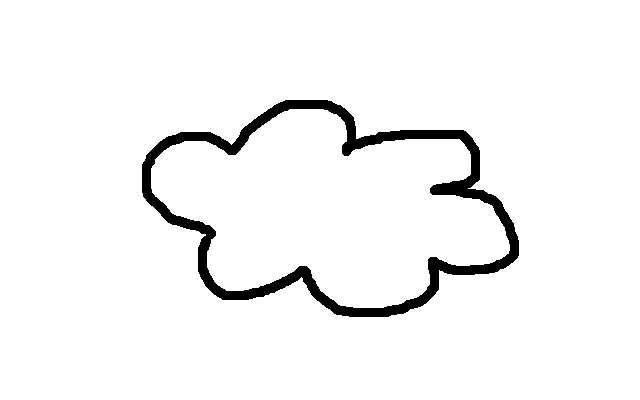
\includegraphics[scale = 0.5]{cloud}
	\centering
	\caption{Example of drawing}
	\label{fig:cloud}
\end{figure}

In the Figure \ref{fig:cloud} exemplary output image was shown. It is not the exact set of coordinates that was sent to the robot, but only tool that helps user tracking the path of finger's movement. As it was mentioned before commands are sent in the real time and some points drawn in the image were missed. Thus, image made by the robot is more like interpolated and digitized version of an output of finger tracking displayed on the screen.

\subsection{Filter}

One of the objective of this project was to make the leap sensor less sensible to noises. There are many way to do that and many type of existing filters. But as far as our testing went a simple mean filter is more than enough to stabilize the output of the mode 2. The mean filter can be set to work on a diffrent number of position (the ... previous ones).

\begin{figure}[H]
	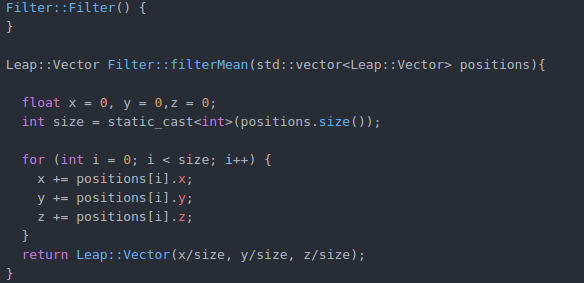
\includegraphics[scale = 0.5]{codeFilter}
	\centering
	\caption{Code of the filter}
	\label{fig:filter}
\end{figure}

Mean filter is easy to implement, but it can cause some issues. The most important thing in this case is a size of buffer - the number by which the sum of coordinates is devided. When that size was too small filter was not working well, cause averaged coordinates were almost the same as that ones giving directly from the leap. On the other, hand bigger size had also one big drawback - hand tracking was very slow and program was not sensitive to the finger movement. After several attempts and combinations proper size was achieved and improvement was easy to see on the screen. 
